\documentclass{article}
\usepackage{tikz}
\usetikzlibrary{shapes.geometric}
\usepackage{subcaption}
\usepackage{geometry}
\geometry{a4paper, margin=1in}

\begin{document}

\begin{figure}[hbt!]
    \centering
    \begin{subfigure}[b]{0.32\textwidth}
        \centering
        \resizebox{\linewidth}{!}{
            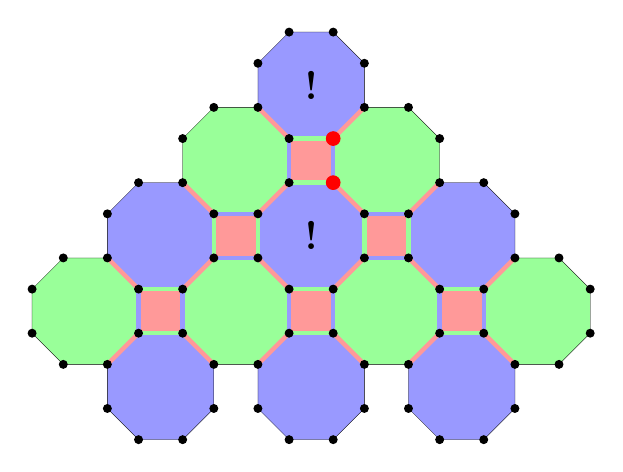
\begin{tikzpicture}[scale=0.7]
    \filldraw[fill=blue!40, draw=black, ultra thin] (-3.6971,-0.4) -- (-3.1314,-0.9657) -- (-2.3314,-0.9657) -- (-1.7657,-0.4) -- (-1.7657,0.4) -- (-2.3314,0.9657) -- (-3.1314,0.9657) -- (-3.6971,0.4) -- cycle;
    \filldraw[fill=blue!40, draw=black, ultra thin] (-0.9657,-0.4) -- (-0.4,-0.9657) -- (0.4,-0.9657) -- (0.9657,-0.4) -- (0.9657,0.4) -- (0.4,0.9657) -- (-0.4,0.9657) -- (-0.9657,0.4) -- cycle;
    \filldraw[fill=blue!40, draw=black, ultra thin] (1.7657,-0.4) -- (2.3314,-0.9657) -- (3.1314,-0.9657) -- (3.6971,-0.4) -- (3.6971,0.4) -- (3.1314,0.9657) -- (2.3314,0.9657) -- (1.7657,0.4) -- cycle;
    \filldraw[fill=green!40, draw=black, ultra thin] (-5.0628,0.9657) -- (-4.4971,0.4) -- (-3.6971,0.4) -- (-3.1314,0.9657) -- (-3.1314,1.7657) -- (-3.6971,2.3314) -- (-4.4971,2.3314) -- (-5.0628,1.7657) -- cycle;
    \filldraw[fill=red!40, draw=black, ultra thin] (-3.1314,0.9657) -- (-2.3314,0.9657) -- (-2.3314,1.7657) -- (-3.1314,1.7657) -- cycle;
    \filldraw[fill=green!40, draw=black, ultra thin] (-2.3314,0.9657) -- (-1.7657,0.4) -- (-0.9657,0.4) -- (-0.4,0.9657) -- (-0.4,1.7657) -- (-0.9657,2.3314) -- (-1.7657,2.3314) -- (-2.3314,1.7657) -- cycle;
    \filldraw[fill=red!40, draw=black, ultra thin] (-0.4,0.9657) -- (0.4,0.9657) -- (0.4,1.7657) -- (-0.4,1.7657) -- cycle;
    \filldraw[fill=green!40, draw=black, ultra thin] (0.4,0.9657) -- (0.9657,0.4) -- (1.7657,0.4) -- (2.3314,0.9657) -- (2.3314,1.7657) -- (1.7657,2.3314) -- (0.9657,2.3314) -- (0.4,1.7657) -- cycle;
    \filldraw[fill=red!40, draw=black, ultra thin] (2.3314,0.9657) -- (3.1314,0.9657) -- (3.1314,1.7657) -- (2.3314,1.7657) -- cycle;
    \filldraw[fill=green!40, draw=black, ultra thin] (3.1314,0.9657) -- (3.6971,0.4) -- (4.4971,0.4) -- (5.0628,0.9657) -- (5.0628,1.7657) -- (4.4971,2.3314) -- (3.6971,2.3314) -- (3.1314,1.7657) -- cycle;
    \filldraw[fill=blue!40, draw=black, ultra thin] (-3.6971,2.3314) -- (-3.1314,1.7657) -- (-2.3314,1.7657) -- (-1.7657,2.3314) -- (-1.7657,3.1314) -- (-2.3314,3.6971) -- (-3.1314,3.6971) -- (-3.6971,3.1314) -- cycle;
    \filldraw[fill=red!40, draw=black, ultra thin] (-1.7657,2.3314) -- (-0.9657,2.3314) -- (-0.9657,3.1314) -- (-1.7657,3.1314) -- cycle;
    \filldraw[fill=blue!40, draw=black, ultra thin] (-0.9657,2.3314) -- (-0.4,1.7657) -- (0.4,1.7657) -- (0.9657,2.3314) -- (0.9657,3.1314) -- (0.4,3.6971) -- (-0.4,3.6971) -- (-0.9657,3.1314) -- cycle;
    \node at (0, 2.7314) {\textbf{\Large !}} ;
    \filldraw[fill=red!40, draw=black, ultra thin] (0.9657,2.3314) -- (1.7657,2.3314) -- (1.7657,3.1314) -- (0.9657,3.1314) -- cycle;
    \filldraw[fill=blue!40, draw=black, ultra thin] (1.7657,2.3314) -- (2.3314,1.7657) -- (3.1314,1.7657) -- (3.6971,2.3314) -- (3.6971,3.1314) -- (3.1314,3.6971) -- (2.3314,3.6971) -- (1.7657,3.1314) -- cycle;
    \filldraw[fill=green!40, draw=black, ultra thin] (-2.3314,3.6971) -- (-1.7657,3.1314) -- (-0.9657,3.1314) -- (-0.4,3.6971) -- (-0.4,4.4971) -- (-0.9657,5.0628) -- (-1.7657,5.0628) -- (-2.3314,4.4971) -- cycle;
    \filldraw[fill=red!40, draw=black, ultra thin] (-0.4,3.6971) -- (0.4,3.6971) -- (0.4,4.4971) -- (-0.4,4.4971) -- cycle;
    \filldraw[fill=green!40, draw=black, ultra thin] (0.4,3.6971) -- (0.9657,3.1314) -- (1.7657,3.1314) -- (2.3314,3.6971) -- (2.3314,4.4971) -- (1.7657,5.0628) -- (0.9657,5.0628) -- (0.4,4.4971) -- cycle;
    \filldraw[fill=blue!40, draw=black, ultra thin] (-0.9657,5.0628) -- (-0.4,4.4971) -- (0.4,4.4971) -- (0.9657,5.0628) -- (0.9657,5.8628) -- (0.4,6.4285) -- (-0.4,6.4285) -- (-0.9657,5.8628) -- cycle;
    \node at (0, 5.4628) {\textbf{\Large !}} ;
    \draw[red!40, ultra thick] (-1.7657, 0.4) -- (-2.3314, 0.9657);
    \draw[green!40, ultra thick] (-2.3314, 0.9657) -- (-3.1314, 0.9657);
    \draw[blue!40, ultra thick] (-2.3314, 0.9657) -- (-2.3314, 1.7657);
    \draw[red!40, ultra thick] (-3.1314, 0.9657) -- (-3.6971, 0.4);
    \draw[blue!40, ultra thick] (-3.1314, 0.9657) -- (-3.1314, 1.7657);
    \draw[red!40, ultra thick] (0.9657, 0.4) -- (0.4, 0.9657);
    \draw[green!40, ultra thick] (0.4, 0.9657) -- (-0.4, 0.9657);
    \draw[blue!40, ultra thick] (0.4, 0.9657) -- (0.4, 1.7657);
    \draw[red!40, ultra thick] (-0.4, 0.9657) -- (-0.9657, 0.4);
    \draw[blue!40, ultra thick] (-0.4, 0.9657) -- (-0.4, 1.7657);
    \draw[red!40, ultra thick] (3.6971, 0.4) -- (3.1314, 0.9657);
    \draw[green!40, ultra thick] (3.1314, 0.9657) -- (2.3314, 0.9657);
    \draw[blue!40, ultra thick] (3.1314, 0.9657) -- (3.1314, 1.7657);
    \draw[red!40, ultra thick] (2.3314, 0.9657) -- (1.7657, 0.4);
    \draw[blue!40, ultra thick] (2.3314, 0.9657) -- (2.3314, 1.7657);
    \draw[red!40, ultra thick] (-3.1314, 1.7657) -- (-3.6971, 2.3314);
    \draw[green!40, ultra thick] (-3.1314, 1.7657) -- (-2.3314, 1.7657);
    \draw[red!40, ultra thick] (-2.3314, 1.7657) -- (-1.7657, 2.3314);
    \draw[red!40, ultra thick] (-0.4, 1.7657) -- (-0.9657, 2.3314);
    \draw[green!40, ultra thick] (-0.4, 1.7657) -- (0.4, 1.7657);
    \draw[blue!40, ultra thick] (-0.9657, 2.3314) -- (-1.7657, 2.3314);
    \draw[green!40, ultra thick] (-0.9657, 2.3314) -- (-0.9657, 3.1314);
    \draw[green!40, ultra thick] (-1.7657, 2.3314) -- (-1.7657, 3.1314);
    \draw[red!40, ultra thick] (0.4, 1.7657) -- (0.9657, 2.3314);
    \draw[red!40, ultra thick] (2.3314, 1.7657) -- (1.7657, 2.3314);
    \draw[green!40, ultra thick] (2.3314, 1.7657) -- (3.1314, 1.7657);
    \draw[blue!40, ultra thick] (1.7657, 2.3314) -- (0.9657, 2.3314);
    \draw[green!40, ultra thick] (1.7657, 2.3314) -- (1.7657, 3.1314);
    \draw[green!40, ultra thick] (0.9657, 2.3314) -- (0.9657, 3.1314);
    \draw[red!40, ultra thick] (3.1314, 1.7657) -- (3.6971, 2.3314);
    \draw[red!40, ultra thick] (-1.7657, 3.1314) -- (-2.3314, 3.6971);
    \draw[blue!40, ultra thick] (-1.7657, 3.1314) -- (-0.9657, 3.1314);
    \draw[red!40, ultra thick] (-0.9657, 3.1314) -- (-0.4, 3.6971);
    \draw[red!40, ultra thick] (0.9657, 3.1314) -- (0.4, 3.6971);
    \draw[blue!40, ultra thick] (0.9657, 3.1314) -- (1.7657, 3.1314);
    \draw[green!40, ultra thick] (0.4, 3.6971) -- (-0.4, 3.6971);
    \draw[blue!40, ultra thick] (0.4, 3.6971) -- (0.4, 4.4971);
    \draw[blue!40, ultra thick] (-0.4, 3.6971) -- (-0.4, 4.4971);
    \draw[red!40, ultra thick] (1.7657, 3.1314) -- (2.3314, 3.6971);
    \draw[red!40, ultra thick] (-0.4, 4.4971) -- (-0.9657, 5.0628);
    \draw[green!40, ultra thick] (-0.4, 4.4971) -- (0.4, 4.4971);
    \draw[red!40, ultra thick] (0.4, 4.4971) -- (0.9657, 5.0628);
    \filldraw[black] (-3.1314, -0.9657) circle (2pt);
    \filldraw[black] (-2.3314, -0.9657) circle (2pt);
    \filldraw[black] (-1.7657, -0.4) circle (2pt);
    \filldraw[black] (-1.7657, 0.4) circle (2pt);
    \filldraw[black] (-2.3314, 0.9657) circle (2pt);
    \filldraw[black] (-3.1314, 0.9657) circle (2pt);
    \filldraw[black] (-3.6971, 0.4) circle (2pt);
    \filldraw[black] (-3.6971, -0.4) circle (2pt);
    \filldraw[black] (-0.4, -0.9657) circle (2pt);
    \filldraw[black] (0.4, -0.9657) circle (2pt);
    \filldraw[black] (0.9657, -0.4) circle (2pt);
    \filldraw[black] (0.9657, 0.4) circle (2pt);
    \filldraw[black] (0.4, 0.9657) circle (2pt);
    \filldraw[black] (-0.4, 0.9657) circle (2pt);
    \filldraw[black] (-0.9657, 0.4) circle (2pt);
    \filldraw[black] (-0.9657, -0.4) circle (2pt);
    \filldraw[black] (2.3314, -0.9657) circle (2pt);
    \filldraw[black] (3.1314, -0.9657) circle (2pt);
    \filldraw[black] (3.6971, -0.4) circle (2pt);
    \filldraw[black] (3.6971, 0.4) circle (2pt);
    \filldraw[black] (3.1314, 0.9657) circle (2pt);
    \filldraw[black] (2.3314, 0.9657) circle (2pt);
    \filldraw[black] (1.7657, 0.4) circle (2pt);
    \filldraw[black] (1.7657, -0.4) circle (2pt);
    \filldraw[black] (-4.4971, 0.4) circle (2pt);
    \filldraw[black] (-3.1314, 1.7657) circle (2pt);
    \filldraw[black] (-3.6971, 2.3314) circle (2pt);
    \filldraw[black] (-4.4971, 2.3314) circle (2pt);
    \filldraw[black] (-5.0628, 1.7657) circle (2pt);
    \filldraw[black] (-5.0628, 0.9657) circle (2pt);
    \filldraw[black] (-2.3314, 1.7657) circle (2pt);
    \filldraw[black] (-0.4, 1.7657) circle (2pt);
    \filldraw[black] (-0.9657, 2.3314) circle (2pt);
    \filldraw[black] (-1.7657, 2.3314) circle (2pt);
    \filldraw[black] (0.4, 1.7657) circle (2pt);
    \filldraw[black] (2.3314, 1.7657) circle (2pt);
    \filldraw[black] (1.7657, 2.3314) circle (2pt);
    \filldraw[black] (0.9657, 2.3314) circle (2pt);
    \filldraw[black] (3.1314, 1.7657) circle (2pt);
    \filldraw[black] (4.4971, 0.4) circle (2pt);
    \filldraw[black] (5.0628, 0.9657) circle (2pt);
    \filldraw[black] (5.0628, 1.7657) circle (2pt);
    \filldraw[black] (4.4971, 2.3314) circle (2pt);
    \filldraw[black] (3.6971, 2.3314) circle (2pt);
    \filldraw[black] (-1.7657, 3.1314) circle (2pt);
    \filldraw[black] (-2.3314, 3.6971) circle (2pt);
    \filldraw[black] (-3.1314, 3.6971) circle (2pt);
    \filldraw[black] (-3.6971, 3.1314) circle (2pt);
    \filldraw[black] (-0.9657, 3.1314) circle (2pt);
    \filldraw[black] (0.9657, 3.1314) circle (2pt);
    \filldraw[red] (0.4, 3.6971) circle (3.5pt);
    \filldraw[black] (-0.4, 3.6971) circle (2pt);
    \filldraw[black] (1.7657, 3.1314) circle (2pt);
    \filldraw[black] (3.6971, 3.1314) circle (2pt);
    \filldraw[black] (3.1314, 3.6971) circle (2pt);
    \filldraw[black] (2.3314, 3.6971) circle (2pt);
    \filldraw[black] (-0.4, 4.4971) circle (2pt);
    \filldraw[black] (-0.9657, 5.0628) circle (2pt);
    \filldraw[black] (-1.7657, 5.0628) circle (2pt);
    \filldraw[black] (-2.3314, 4.4971) circle (2pt);
    \filldraw[red] (0.4, 4.4971) circle (3.5pt);
    \filldraw[black] (2.3314, 4.4971) circle (2pt);
    \filldraw[black] (1.7657, 5.0628) circle (2pt);
    \filldraw[black] (0.9657, 5.0628) circle (2pt);
    \filldraw[black] (0.9657, 5.8628) circle (2pt);
    \filldraw[black] (0.4, 6.4285) circle (2pt);
    \filldraw[black] (-0.4, 6.4285) circle (2pt);
    \filldraw[black] (-0.9657, 5.8628) circle (2pt);
\end{tikzpicture}

        }
        \caption{Active detectors}
        \label{fig:concat_exec_syndrome}
    \end{subfigure}
    \hfill
    \begin{subfigure}[b]{0.32\textwidth}
        \centering
        \resizebox{\linewidth}{!}{
            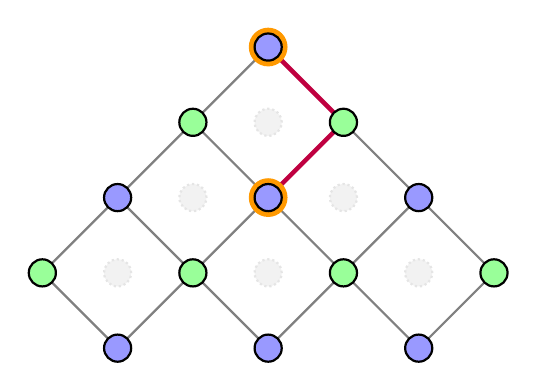
\begin{tikzpicture}[scale=0.7]
    \draw[gray, thick] (-1.3657, 1.3657) -- (-2.7314, 0);
    \draw[gray, thick] (-4.0971, 1.3657) -- (-2.7314, 0);
    \draw[gray, thick] (1.3657, 1.3657) -- (0, 0);
    \draw[gray, thick] (-1.3657, 1.3657) -- (0, 0);
    \draw[gray, thick] (4.0971, 1.3657) -- (2.7314, 0);
    \draw[gray, thick] (1.3657, 1.3657) -- (2.7314, 0);
    \draw[gray, thick] (-4.0971, 1.3657) -- (-2.7314, 2.7314);
    \draw[gray, thick] (-1.3657, 1.3657) -- (-2.7314, 2.7314);
    \draw[gray, thick] (-1.3657, 1.3657) -- (0, 2.7314);
    \draw[gray, thick] (1.3657, 1.3657) -- (0, 2.7314);
    \draw[gray, thick] (1.3657, 1.3657) -- (2.7314, 2.7314);
    \draw[gray, thick] (4.0971, 1.3657) -- (2.7314, 2.7314);
    \draw[gray, thick] (-1.3657, 4.0971) -- (-2.7314, 2.7314);
    \draw[gray, thick] (-1.3657, 4.0971) -- (0, 2.7314);
    \draw[purple, ultra thick] (1.3657, 4.0971) -- (0, 2.7314);
    \draw[gray, thick] (1.3657, 4.0971) -- (2.7314, 2.7314);
    \draw[gray, thick] (-1.3657, 4.0971) -- (0, 5.4628);
    \draw[purple, ultra thick] (1.3657, 4.0971) -- (0, 5.4628);
    \filldraw[fill=blue!40, draw=black, thick] (-2.7314, 0) circle (7pt);
    \filldraw[fill=blue!40, draw=black, thick] (0, 0) circle (7pt);
    \filldraw[fill=blue!40, draw=black, thick] (2.7314, 0) circle (7pt);
    \filldraw[fill=green!40, draw=black, thick] (-4.0971, 1.3657) circle (7pt);
    \filldraw[fill=gray!10, draw=gray!20, densely dotted, thick] (-2.7314, 1.3657) circle (7pt);
    \filldraw[fill=green!40, draw=black, thick] (-1.3657, 1.3657) circle (7pt);
    \filldraw[fill=gray!10, draw=gray!20, densely dotted, thick] (0, 1.3657) circle (7pt);
    \filldraw[fill=green!40, draw=black, thick] (1.3657, 1.3657) circle (7pt);
    \filldraw[fill=gray!10, draw=gray!20, densely dotted, thick] (2.7314, 1.3657) circle (7pt);
    \filldraw[fill=green!40, draw=black, thick] (4.0971, 1.3657) circle (7pt);
    \filldraw[fill=blue!40, draw=black, thick] (-2.7314, 2.7314) circle (7pt);
    \filldraw[fill=gray!10, draw=gray!20, densely dotted, thick] (-1.3657, 2.7314) circle (7pt);
    \filldraw[fill=orange!80!yellow, draw=none] (0, 2.7314) circle (10pt);
    \filldraw[fill=blue!40, draw=black, thick] (0, 2.7314) circle (7pt);
    \filldraw[fill=gray!10, draw=gray!20, densely dotted, thick] (1.3657, 2.7314) circle (7pt);
    \filldraw[fill=blue!40, draw=black, thick] (2.7314, 2.7314) circle (7pt);
    \filldraw[fill=green!40, draw=black, thick] (-1.3657, 4.0971) circle (7pt);
    \filldraw[fill=gray!10, draw=gray!20, densely dotted, thick] (0, 4.0971) circle (7pt);
    \filldraw[fill=green!40, draw=black, thick] (1.3657, 4.0971) circle (7pt);
    \filldraw[fill=orange!80!yellow, draw=none] (0, 5.4628) circle (10pt);
    \filldraw[fill=blue!40, draw=black, thick] (0, 5.4628) circle (7pt);
\end{tikzpicture}

        }
        \caption{First-round MWPM}
        \label{fig:concat_exec_mwpm1}
    \end{subfigure}
    \hfill
    \begin{subfigure}[b]{0.32\textwidth}
        \centering
        \resizebox{\linewidth}{!}{
            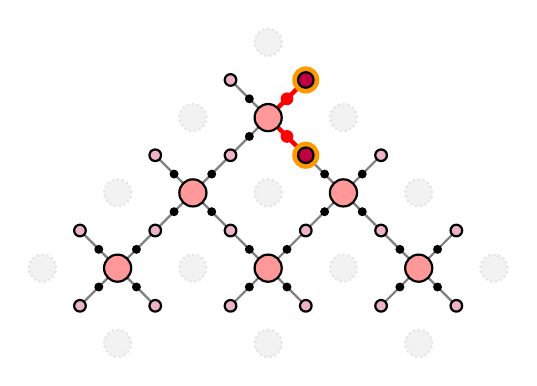
\begin{tikzpicture}[scale=0.7]
    \draw[gray, thick] (-2.7314, 1.3657) -- (-2.0486, 0.6828);
    \filldraw[black] (-2.39, 1.0242) circle (2pt);
    \filldraw[fill=purple!30, draw=black, thick] (-2.0486, 0.6828) circle (3pt);
    \draw[gray, thick] (-2.7314, 1.3657) -- (-3.4143, 0.6828);
    \filldraw[black] (-3.0728, 1.0242) circle (2pt);
    \filldraw[fill=purple!30, draw=black, thick] (-3.4143, 0.6828) circle (3pt);
    \draw[gray, thick] (0, 1.3657) -- (0.6828, 0.6828);
    \filldraw[black] (0.3414, 1.0242) circle (2pt);
    \filldraw[fill=purple!30, draw=black, thick] (0.6828, 0.6828) circle (3pt);
    \draw[gray, thick] (0, 1.3657) -- (-0.6828, 0.6828);
    \filldraw[black] (-0.3414, 1.0242) circle (2pt);
    \filldraw[fill=purple!30, draw=black, thick] (-0.6828, 0.6828) circle (3pt);
    \draw[gray, thick] (2.7314, 1.3657) -- (3.4143, 0.6828);
    \filldraw[black] (3.0728, 1.0242) circle (2pt);
    \filldraw[fill=purple!30, draw=black, thick] (3.4143, 0.6828) circle (3pt);
    \draw[gray, thick] (2.7314, 1.3657) -- (2.0486, 0.6828);
    \filldraw[black] (2.39, 1.0242) circle (2pt);
    \filldraw[fill=purple!30, draw=black, thick] (2.0486, 0.6828) circle (3pt);
    \draw[gray, thick] (-2.7314, 1.3657) -- (-3.4143, 2.0486);
    \filldraw[black] (-3.0728, 1.7071) circle (2pt);
    \filldraw[fill=purple!30, draw=black, thick] (-3.4143, 2.0486) circle (3pt);
    \draw[gray, thick] (-2.7314, 1.3657) -- (-2.0486, 2.0486);
    \filldraw[black] (-2.39, 1.7071) circle (2pt);
    \draw[gray, thick] (-1.3657, 2.7314) -- (-2.0486, 2.0486);
    \filldraw[black] (-1.7071, 2.39) circle (2pt);
    \filldraw[fill=purple!30, draw=black, thick] (-2.0486, 2.0486) circle (3pt);
    \draw[gray, thick] (0, 1.3657) -- (-0.6828, 2.0486);
    \filldraw[black] (-0.3414, 1.7071) circle (2pt);
    \draw[gray, thick] (-1.3657, 2.7314) -- (-0.6828, 2.0486);
    \filldraw[black] (-1.0242, 2.39) circle (2pt);
    \filldraw[fill=purple!30, draw=black, thick] (-0.6828, 2.0486) circle (3pt);
    \draw[gray, thick] (0, 1.3657) -- (0.6828, 2.0486);
    \filldraw[black] (0.3414, 1.7071) circle (2pt);
    \draw[gray, thick] (1.3657, 2.7314) -- (0.6828, 2.0486);
    \filldraw[black] (1.0242, 2.39) circle (2pt);
    \filldraw[fill=purple!30, draw=black, thick] (0.6828, 2.0486) circle (3pt);
    \draw[gray, thick] (2.7314, 1.3657) -- (2.0486, 2.0486);
    \filldraw[black] (2.39, 1.7071) circle (2pt);
    \draw[gray, thick] (1.3657, 2.7314) -- (2.0486, 2.0486);
    \filldraw[black] (1.7071, 2.39) circle (2pt);
    \filldraw[fill=purple!30, draw=black, thick] (2.0486, 2.0486) circle (3pt);
    \draw[gray, thick] (2.7314, 1.3657) -- (3.4143, 2.0486);
    \filldraw[black] (3.0728, 1.7071) circle (2pt);
    \filldraw[fill=purple!30, draw=black, thick] (3.4143, 2.0486) circle (3pt);
    \draw[gray, thick] (-1.3657, 2.7314) -- (-2.0486, 3.4143);
    \filldraw[black] (-1.7071, 3.0728) circle (2pt);
    \filldraw[fill=purple!30, draw=black, thick] (-2.0486, 3.4143) circle (3pt);
    \draw[gray, thick] (-1.3657, 2.7314) -- (-0.6828, 3.4143);
    \filldraw[black] (-1.0242, 3.0728) circle (2pt);
    \draw[gray, thick] (0, 4.0971) -- (-0.6828, 3.4143);
    \filldraw[black] (-0.3414, 3.7557) circle (2pt);
    \filldraw[fill=purple!30, draw=black, thick] (-0.6828, 3.4143) circle (3pt);
    \draw[gray, thick] (1.3657, 2.7314) -- (0.6828, 3.4143);
    \filldraw[black] (1.0242, 3.0728) circle (2pt);
    \draw[red, ultra thick] (0, 4.0971) -- (0.6828, 3.4143);
    \filldraw[red] (0.3414, 3.7557) circle (3pt);
    \filldraw[fill=orange!80!yellow, draw=none] (0.6828, 3.4143) circle (7pt);
    \filldraw[fill=purple, draw=black, thick] (0.6828, 3.4143) circle (4pt);
    \draw[gray, thick] (1.3657, 2.7314) -- (2.0486, 3.4143);
    \filldraw[black] (1.7071, 3.0728) circle (2pt);
    \filldraw[fill=purple!30, draw=black, thick] (2.0486, 3.4143) circle (3pt);
    \draw[gray, thick] (0, 4.0971) -- (-0.6828, 4.7799);
    \filldraw[black] (-0.3414, 4.4385) circle (2pt);
    \filldraw[fill=purple!30, draw=black, thick] (-0.6828, 4.7799) circle (3pt);
    \draw[red, ultra thick] (0, 4.0971) -- (0.6828, 4.7799);
    \filldraw[red] (0.3414, 4.4385) circle (3pt);
    \filldraw[fill=orange!80!yellow, draw=none] (0.6828, 4.7799) circle (7pt);
    \filldraw[fill=purple, draw=black, thick] (0.6828, 4.7799) circle (4pt);
    \filldraw[fill=gray!10, draw=gray!20, densely dotted, thick] (-2.7314, 0) circle (7pt);
    \filldraw[fill=gray!10, draw=gray!20, densely dotted, thick] (0, 0) circle (7pt);
    \filldraw[fill=gray!10, draw=gray!20, densely dotted, thick] (2.7314, 0) circle (7pt);
    \filldraw[fill=gray!10, draw=gray!20, densely dotted, thick] (-4.0971, 1.3657) circle (7pt);
    \filldraw[fill=red!40, draw=black, thick] (-2.7314, 1.3657) circle (7pt);
    \filldraw[fill=gray!10, draw=gray!20, densely dotted, thick] (-1.3657, 1.3657) circle (7pt);
    \filldraw[fill=red!40, draw=black, thick] (0, 1.3657) circle (7pt);
    \filldraw[fill=gray!10, draw=gray!20, densely dotted, thick] (1.3657, 1.3657) circle (7pt);
    \filldraw[fill=red!40, draw=black, thick] (2.7314, 1.3657) circle (7pt);
    \filldraw[fill=gray!10, draw=gray!20, densely dotted, thick] (4.0971, 1.3657) circle (7pt);
    \filldraw[fill=gray!10, draw=gray!20, densely dotted, thick] (-2.7314, 2.7314) circle (7pt);
    \filldraw[fill=red!40, draw=black, thick] (-1.3657, 2.7314) circle (7pt);
    \filldraw[fill=gray!10, draw=gray!20, densely dotted, thick] (0, 2.7314) circle (7pt);
    \filldraw[fill=red!40, draw=black, thick] (1.3657, 2.7314) circle (7pt);
    \filldraw[fill=gray!10, draw=gray!20, densely dotted, thick] (2.7314, 2.7314) circle (7pt);
    \filldraw[fill=gray!10, draw=gray!20, densely dotted, thick] (-1.3657, 4.0971) circle (7pt);
    \filldraw[fill=red!40, draw=black, thick] (0, 4.0971) circle (7pt);
    \filldraw[fill=gray!10, draw=gray!20, densely dotted, thick] (1.3657, 4.0971) circle (7pt);
    \filldraw[fill=gray!10, draw=gray!20, densely dotted, thick] (0, 5.4628) circle (7pt);
\end{tikzpicture}

        }
        \caption{Second-round MWPM}
        \label{fig:concat_exec_mwpm2}
    \end{subfigure}
    
    \caption[Decoding flow of the Concatenated MWPM Red sub-routine.]{Decoding flow of the Concatenated MWPM Red sub-routine. \textbf{(a)} An error string of two physical qubits (red dots) triggers two Green, two Blue, and no Red detectors (highlighted in glowing orange). \textbf{(b)} First-round MWPM: The active Green and Blue detectors are perfectly matched in the Red-restricted lattice, successfully identifying the faulty Red edge (thick purple line). \textbf{(c)} Second-round MWPM: The previously identified Red edge is mapped as an active defect (purple node with orange glow) in the Red-only lattice, along with any active Red detectors (none in this example). The final matching correctly identifies the exact physical qubits (thick orange lines) that caused the syndrome.}
    \label{fig:4:concatenated_execution}
\end{figure}

\end{document}
